\chapter{大动量希格斯粒子和XWW共振态的物理和研究动机}
\label{chap2}
\fontsize{12bp}{14.4pt}

\section{希格斯粒子的产生和衰变}
在标准模型中,夸克、轻子、W、Z玻色子都通过希格斯机制被赋予质量。LHC以及下一代对撞机实验的重要目标之一就是研究测量希格斯粒子的相关性质,因此,对LHC上希格斯粒子的产生和衰变测量本身就是极为重要的一个任务。

本节除了讨论希格斯粒子的产生和衰变,还将讨论LHC上大动量希格斯粒子的物理特性和研究动机,并且指出我们感兴趣的$X\to WW$共振态搜寻的物理背景和动机(包括标准模型的希格斯粒子以及非标准模型的共振态)
\subsection{希格斯粒子的产生}
LHC上标准模型希格斯粒子的产生道如下\textbf{表\ref{table:2.1}}所示
\begin{table}[htbp]
    \caption{标准模型中希格斯粒子的产生道和相关参数\cite{Higgs_cross_sections}}\label{table:2.1}
    \centering
    \begin{tabular}{>{\centering\arraybackslash}p{2cm}%
    >{\centering\arraybackslash}p{7cm}%
    >{\centering\arraybackslash}p{2cm}%
    >{\centering\arraybackslash}p{2cm}}
    \toprule\toprule
    \textbf{产生道} & \textbf{产生方式} & \textbf{分支比} & \textbf{截面}\\
    \midrule
    ggF & 胶子通过b/top夸克圈聚合产生 & $\sim 87\%$ & \SI{48.5}{pb}\\
    VBF & W/Z矢量玻色子聚合产生 & $\sim7\%$ & \SI{3.78}{pb}\\
    WH & W/Z矢量玻色子与希格斯联合产生 & $\sim 4\%$ & \SI{1.37}{pb}\\
    ttH & 正反top夸克与希格斯联合产生 & $\sim1\%$ & \SI{0.51}{pb}\\
    bbH & 正反bottom夸克与希格斯联合产生 &  $\sim 1\%$ & \SI{0.49}{pb}\\
    tH & t,b,$q^\prime$与希格斯联合产生 & $\sim 0.1\%$ & \SI{0.09}{pb}\\
    \bottomrule\bottomrule
\end{tabular}
\end{table}\\
每个产生道都有独特的拓扑结构,对于其中的稀有道,尽管很难探测,却是研究超出标准模型物理的重要手段。

\subsection{希格斯粒子的衰变}
标准模型希格斯粒子的衰变道如下\textbf{表\ref{table:2.2}}所示,对于其中五个非稀有衰变道,有以下性质:
\begin{itemize}
    \item $\gamma\gamma$和$ZZ\to4\ell$道:高分辨度和高信噪比,常用来精确测量希格斯质量和微分散射截面。
    \item $WW$道:高分支比,但衰变末态的中微子导致低信噪比和低分辨度。
    \item $\tau\tau$和$bb$道:高分支比,低信噪比,用于直接探测希格斯粒子与费米子的耦合。
\end{itemize}
\begin{table}[htbp]
    \caption{标准模型中希格斯粒子的衰变道和相关参数\cite{Higgs_cross_sections}}\label{table:2.2}
    \centering
    \begin{tabular}{>{\centering\arraybackslash}p{2cm}%
    >{\centering\arraybackslash}p{7cm}%
    >{\centering\arraybackslash}p{2cm}%
    >{\centering\arraybackslash}p{2cm}}
    \toprule\toprule
    \textbf{衰变道} & \textbf{主要衰变方式(领头阶)} & \textbf{分支比} & \textbf{稀有衰变}\\
    \midrule
    $H\to bb$ & 直接衰变 & $\sim 58.1\%$ & 否\\
    $H\to WW$ & 直接衰变,一个在壳一个离壳 & $\sim 21.5\%$ & 否\\
    $H\to\tau\tau$ & 直接衰变 & $\sim 6.26\%$ & 否\\
    $H\to ZZ$ & 直接衰变 & $\sim2.64\%$ & 否\\
    $H\to \gamma\gamma$ & 通过W/t/b/$\tau$圈间接衰变 &  $\sim0.23\%$ & 否\\
    $H\to\mu\mu$ & 直接衰变 & $\sim 0.022\%$ & 是\\
    $H\to Z\gamma$ & 通过W/t/b/$\tau$圈间接衰变 & $\sim 0.154\%$ & 是\\
    $H\to cc$ & 直接衰变 & $\sim2.88\%$ & 是\\
    $H\to gg$ & 通过top/bottom圈间接衰变 & $\sim 8.18\%$ & 是\\
    \bottomrule\bottomrule
\end{tabular}
\end{table}

\section{大动量希格斯粒子的物理特性和研究动机}
对于大动量希格斯粒子的一个重要特征,就是原本在常规希格斯粒子衰变中分开的两个喷注,在大动量希格斯粒子衰变场景下,会合并成一个喷注,如\textbf{图\ref{fig:2.1}}所示,所以,对大动量希格斯粒子的标记和分析都存在很多和常规情况截然不同的地方。
\begin{figure}[H]
 \centering
 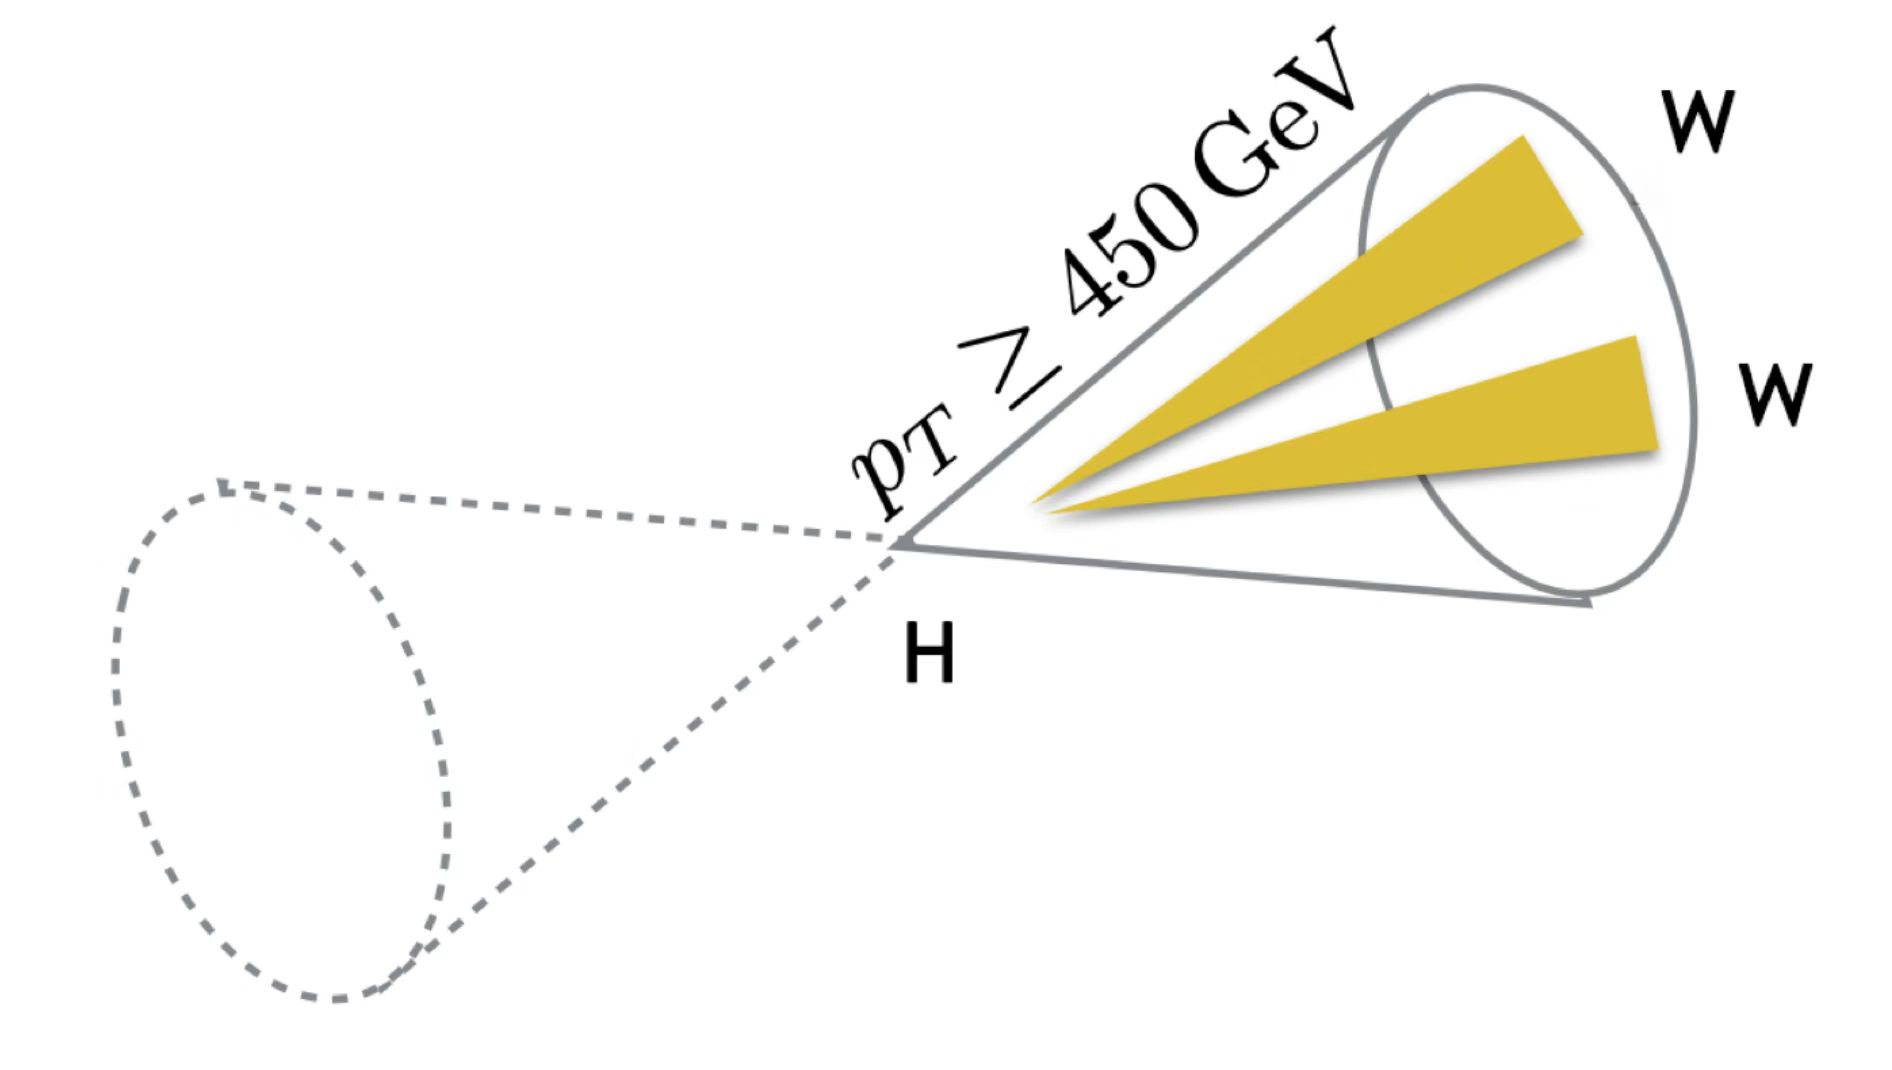
\includegraphics[height=6cm, width=10cm]{pictures/mergedjet.jpg}
  \caption{在动量足够大时,希格斯衰变产物会被重建到同一个喷注中}
 \label{fig:2.1}
\end{figure}

而对大动量希格斯粒子测量有如下物理动机:
\begin{enumerate}
    \item 可以提高标准模型希格斯测量的敏感度:在希格斯粒子$p_T>200$[GeV]的区域,$H\to bb$、$H\to\tau\tau$道还有未分辨出的喷注等待分析;在更高的$p_T$区域,$H\to ZZ/WW\to 4q$道也有同样的需求。
    \item 检验标准模型在大动量区域的高阶修正的正确性或者发现可能的新物理算符。
    \item 可以用作搜寻超出标准模型新物理的工具,包括:辐射子,Randall-Sundrum Bulk Graviton,复合希格斯粒子,新的矢量玻色子三重态,暗物质的探寻(2HDM)等。
\end{enumerate}

\begin{figure}[H]
 \centering
 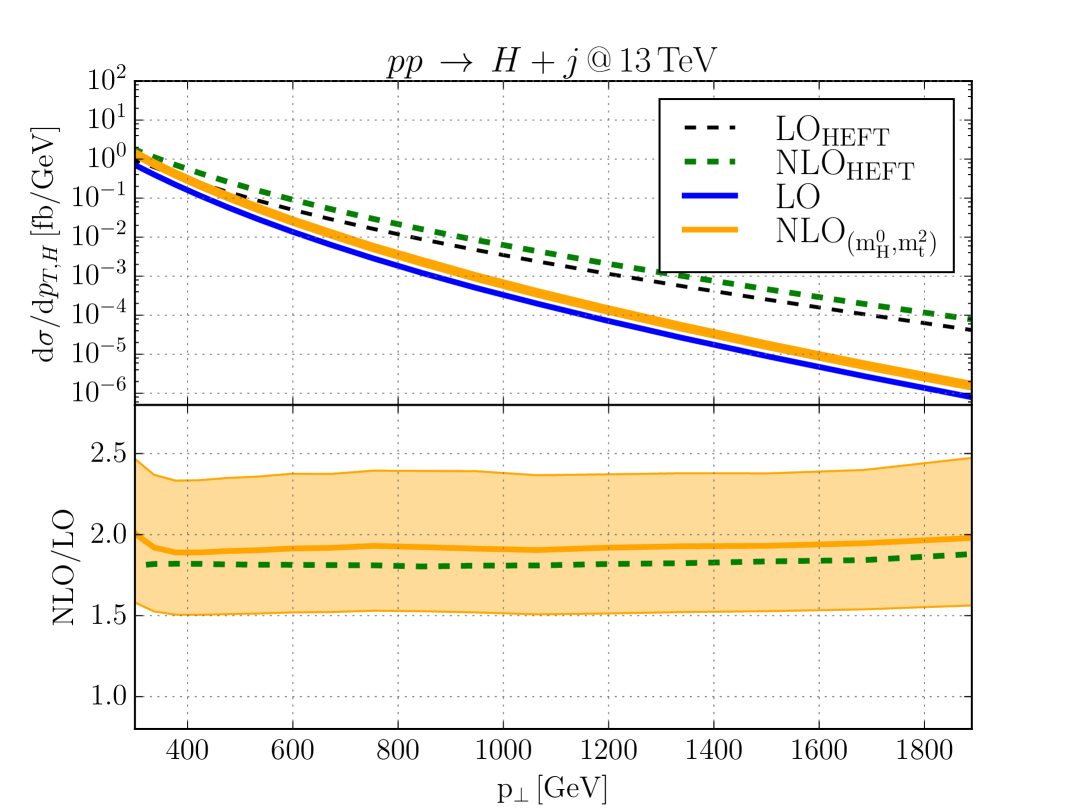
\includegraphics[height=8cm, width=11cm]{pictures/SM_NLO:LO.png}
  \caption{LHC上质心系能量为13TeV时希格斯玻色子的横向动量分布。上图显示标准模型和无穷大top质量有效场论(HEFT)中领头阶(LO)和次领头阶(NLO)的预测。下半部分显示了各自的NLO/LO校准比值。黄色边带表示由于尺度变化导致的标准模型结果的理论误差。\cite{Higgs_high_pt}}
 \label{fig:2.2}
\end{figure}

对于希格斯粒子的大动量区域,唯象上有以下结论\cite{Higgs_high_pt}:标准模型对希格斯粒子动量微分截面的高阶修正在高动量区十分稳定,次领头阶与领头阶的比值固定在一定值范围内(如上\textbf{图\ref{fig:2.1}}所示);而部分超标准模型理论\cite{Higgs_high_pt_BSM}的这一比值则会随动量增大而发生较大的增长(如下\textbf{图\ref{fig:2.2}}所示)。
\begin{figure}[H]
 \centering
 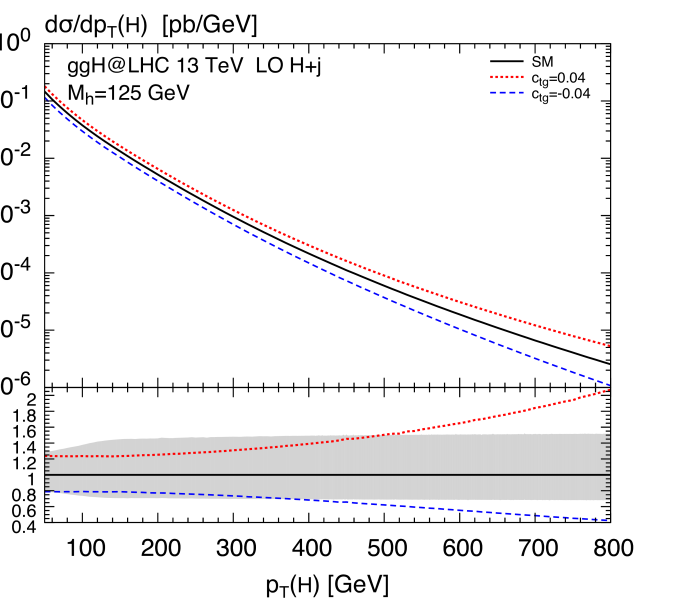
\includegraphics[height=9cm, width=9.8cm]{pictures/BSM_NLO:LO.png}
  \caption{超标准模型的chromomagnetic算符对实验允许范围内的希格斯玻色子谱分布。\cite{Higgs_high_pt_BSM}}
 \label{fig:2.3}
\end{figure}
所以对大动量区域希格斯粒子的搜寻和研究可以用来检验标准模型的精确性以及提供支持/反对新物理的证据。

除此之外,对大动量希格斯玻色子的搜寻还与其他新物理密切相关,比如测量希格斯粒子的属性与标准模型预言的偏差,有助于探索暗物质的性质和物质-反物质不对称性等谜团,因为高能标尺度的新物理无法在大型强子对撞机上直接观察到,但是,在量子场论中,高能标的新物理会间接产生虚粒子,从而导致产生的希格斯玻色子数量作为$p_T$的函数与标准模型会出现较大偏差。这也是我们研究大动量希格斯粒子的一个重要原因:间接地估计高能标尺度上的新物理敏感性。。

\section{$X\to WW$的物理背景及搜寻动机}
WW过程是LHC上第一批可观测到的双玻色子末态之一,而研究WW末态的最原始动机就是搜寻希格斯玻⾊⼦。当下,在CMS实验的RUN III即将开启运行和未来高通量LHC的展望下,我们研究WW共振态的目的就变成了对标准模型希格斯粒子的精确测量和搜寻超标准模型的新WW共振态。
\subsection{标准模型的$H\to WW$}
对于标准模型的$H\to WW$过程,衰变产物为一个质量在壳的$W$和一个质量离壳的$W^*$。所以也常写作$H\to WW^*$。
\begin{figure}[H]
 \centering
 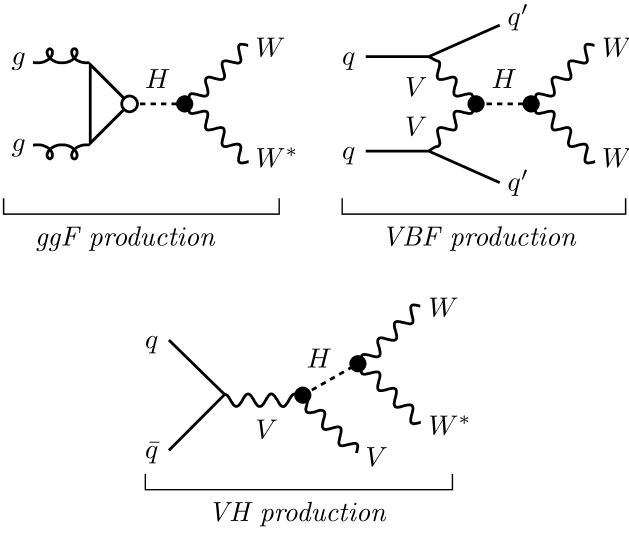
\includegraphics[height=8cm, width=10cm]{pictures/HWW_production.png}
  \caption{$H\to WW$的主要生产过程的领头阶费曼图:(a)通过夸克圈的ggF生产过程;(b)VBF生产过程,末态除了两个W玻色子之外还有两个夸克喷注;(c)VH联合产生,末态有三个玻色子}
 \label{fig:2.4}
\end{figure}
LHC上最多的$H\to WW$产生过程就是胶子聚合产生(ggF),如\textbf{图\ref{fig:2.4}左上}所示。初态胶子通过top夸克圈耦合成希格斯粒子,然后希格斯粒子继续衰变成一对W玻色子。次多产生模式是矢量玻色子聚合产生(VBF),如\textbf{图\ref{fig:2.4}右上}所示,其生产截面大约比ggF小一个数量级。两个初态夸克辐射出W或Z玻色子,然后W或Z玻色子聚合成希格斯粒子,并进一步衰变成一对W玻色子。但VBF末态会生成两个喷注加一对W玻色子,而ggF只会生成一对W玻色子。

$H\to WW^*$的主要本底来自于标准模型下的非共振WW生产道连续谱。在LHC上,WW生产过程由$q\bar{q}$湮灭过程主导\cite{john-alison},如\textbf{图\ref{fig:2.5}}所示:左边和中间分别是$qq^\prime\to WW$过程的t通道图、s通道图,其中s通道过程对于$WWZ$和$WW\gamma$的三玻色子耦合顶点十分敏感。次领头阶的WW本底还有如右边所示的胶子聚合(ggF)生成WW的box图,尽管是次领头阶图,但这个过程被LHC上的高亮度胶子产物增强,从而对非共振态WW的产生贡献也不可忽视。
\begin{figure}[H]
 \centering
 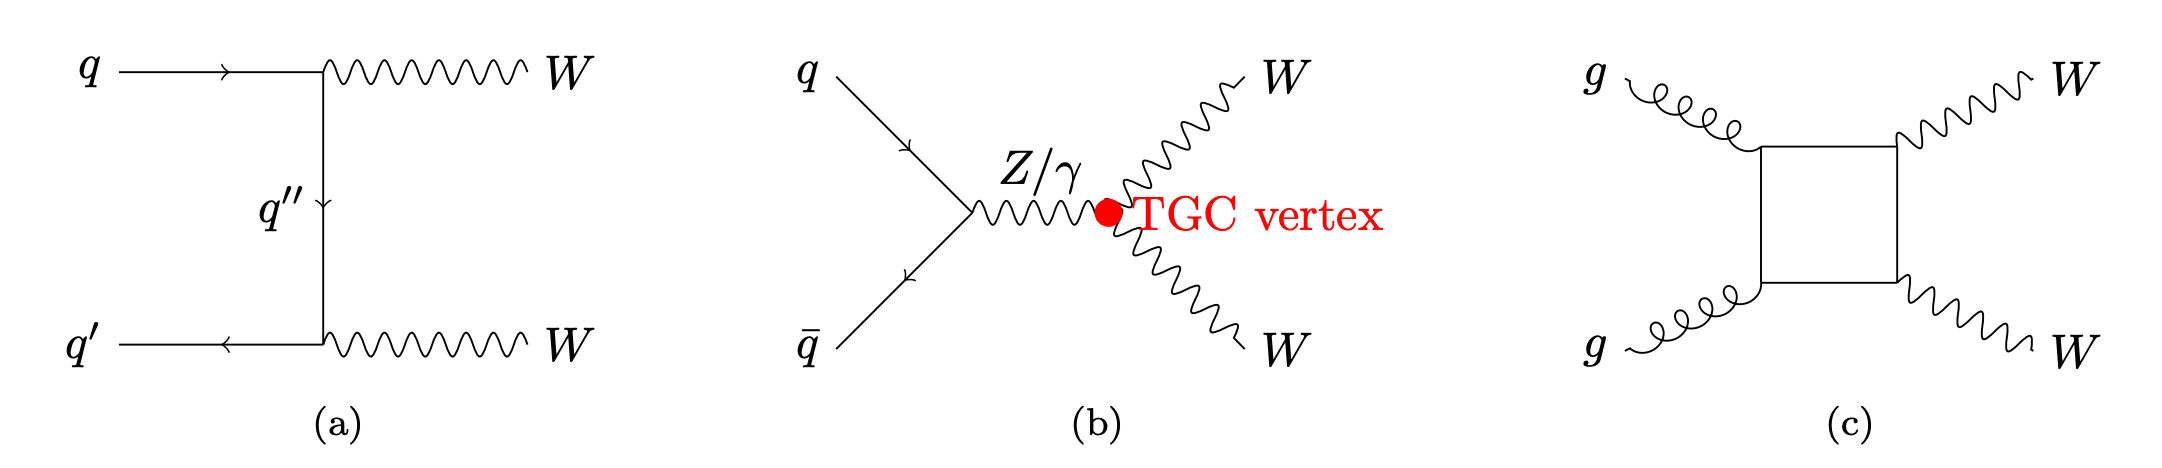
\includegraphics[height=4cm, width=16cm]{pictures/WW_bkg.png}
  \caption{标准模型非共振态$WW$的主要产生过程\cite{john-alison}:(a)$qq^\prime\to WW$的t通道图;(b)$qq^\prime\to WW$的s通道图,有一个三规范玻色子耦合顶点(TGC);(c)$gg\to WW$的box图,贡献被LHC的高亮度胶子抬高。}
 \label{fig:2.5}
\end{figure}

在标准模型框架下,研究双玻色子产生提供了在TeV尺度检验标准模型电弱理论的机会。WW过程就是其中重要的一个例子。除了$H\to WW$产生之外之外,WW产生过程还对三玻色子耦合顶点十分敏感(如\textbf{图\ref{fig:2.5}(b)}所示),从而提供了检验标准模型规范对称性(关于三玻色子耦合限制)的重要机会。通过对WW产生过程的三玻色子耦合的精确测量,我们有机会探寻到包含规范玻色子的新物理现象。(见\ref{sec:2.3.2}节)

\subsection{超标准模型的$X\to WW$}\label{sec:2.3.2}
对于标准模型的$H\to WW$共振态和更重质量的$WW$共振态X,它们的喷注重建也存在区别,如下图所示,重质量的XWW共振态会产生大动量的W玻色子从而导致每个W衰变的两夸克喷注被重建在同一个W喷注里。
\begin{figure}[H]
 \centering
 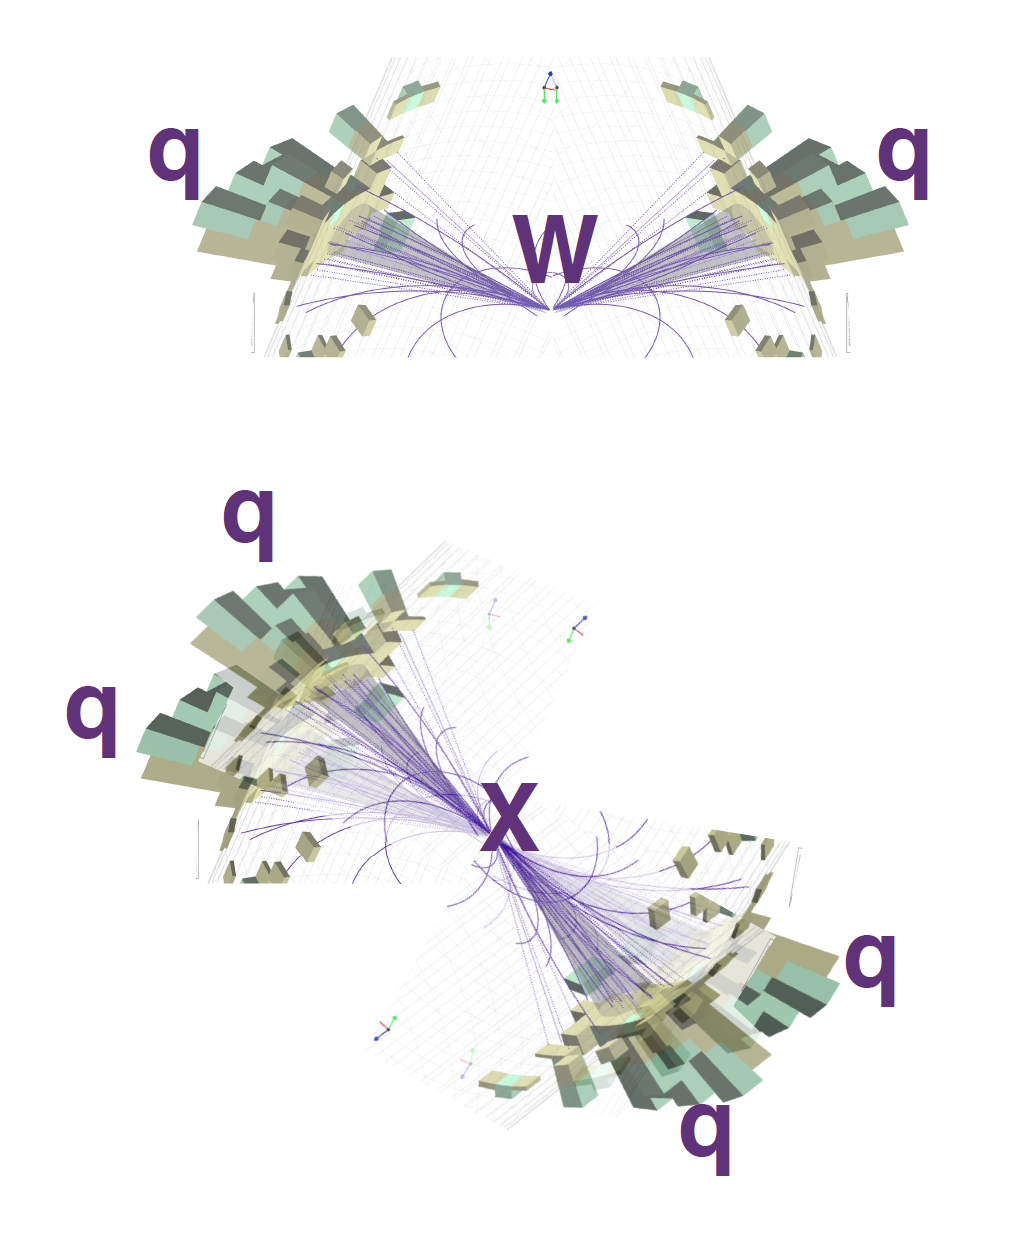
\includegraphics[height=13cm, width=10cm]{pictures/massiveXWW.png}
  \caption{低$p_T$的W玻色子衰变出的两个夸克会被重建为两个喷注,重质量的XWW共振态会产生两个大动量的W玻色子从而导致每个W衰变的两夸克被重建合并为一个喷注。\cite{Boosting_the_Higgs_boson}}
 \label{fig:2.6}
\end{figure}

在这样的物理背景下,对超标准模型的XWW共振态搜寻有助于探寻$V_{kk}$等重质量新物理粒子,如下\textbf{图\ref{fig:2.7}}所示
\begin{figure}[H]
 \centering
 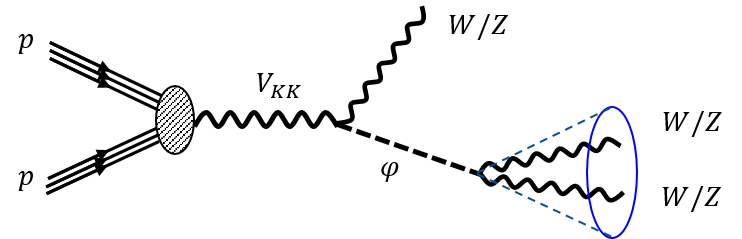
\includegraphics[height=5cm, width=16cm]{pictures/Vkk.png}
  \caption{可考虑的超出标准模型物理过程,基于扭曲的额外维RS模型的扩展。$V_{kk}$表示$W/Z$的Kaluza-Klein(KK)模式,并且对应于较重的母粒子。$\phi$表示标量粒子,被认为是标准模型中的EW规范玻色子。两个$W/Z$粒子周围来自$\phi$衰变的圆锥体表明它们是高度准直的。\cite{Detecting_a_Boosted_Diboson_Resonance}}
 \label{fig:2.7}
\end{figure}

除了对重质量新物理粒子的搜寻,$X\to WW$共振态还可以用来研究非标准模型质量希格斯粒子的衰变分支比关系,如\textbf{图\ref{fig:2.8}}展示了希格斯衰变分支比作为希格斯质量的函数。可以看到双W衰变道在很大的质量范围内都是是最大分支比。特别是当$M_H>130$[GeV]时,就主要是HWW衰变了。在$2m_W<M_H<2m_Z$时,是$H\to WW$分支比非常显著的区间。
\begin{figure}[H]
 \centering
 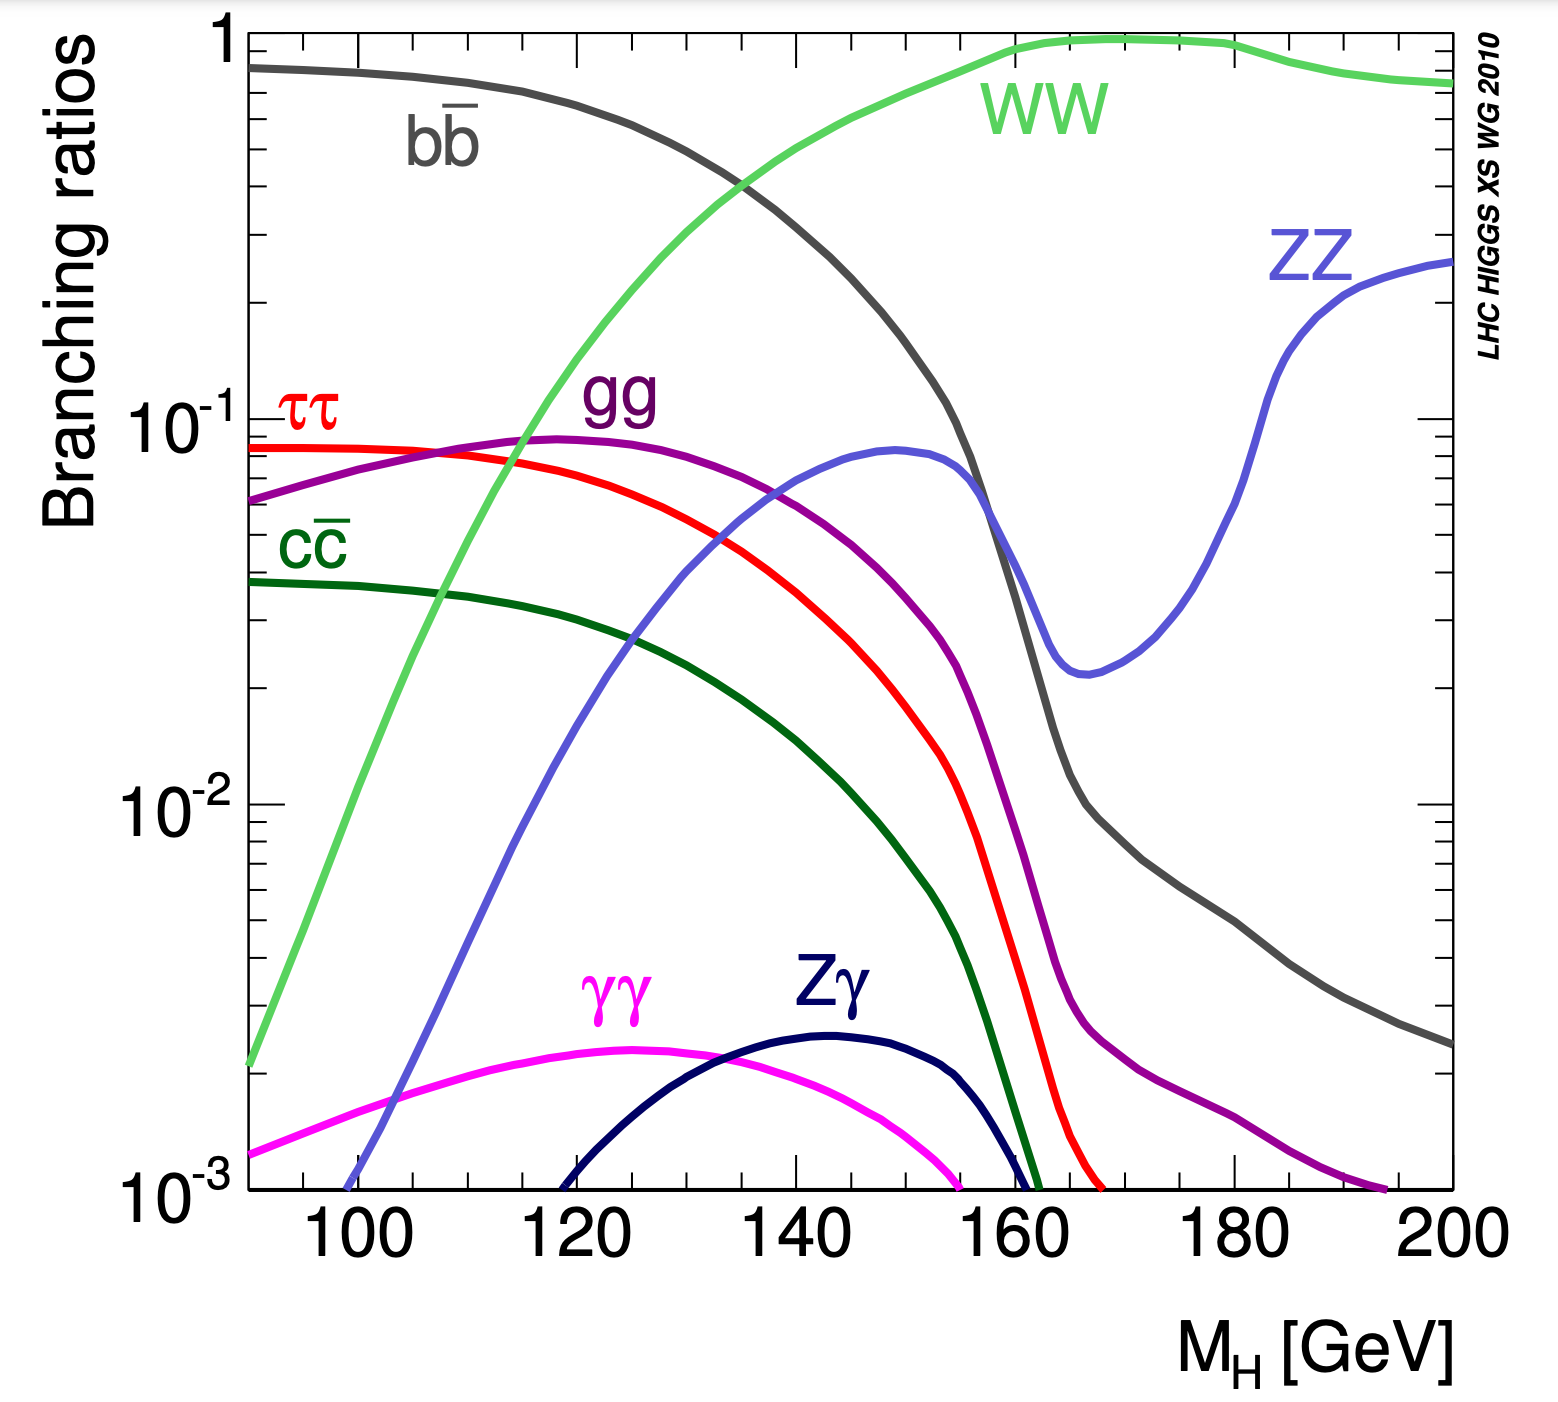
\includegraphics[height=8cm, width=10cm]{pictures/XS-MH.png}
  \caption{不同质量希格斯粒子的衰变分支比}
 \label{fig:2.8}
\end{figure}
因为我们知道$H\to WW$产⽣的速率由希格斯到WW的分⽀⽐决定,所以如果测量得到的$H\to WW$数目与标准模型预言有较大偏差,就暗示着有可能存在着非标准模型质量的伴生/复合希格斯粒子。

如下\textbf{图\ref{fig:2.9}}所示,展示了一种可能的复合希格斯粒子的新物理模型\cite{Boosting_the_Higgs_boson}
\begin{figure}[H]
 \centering
 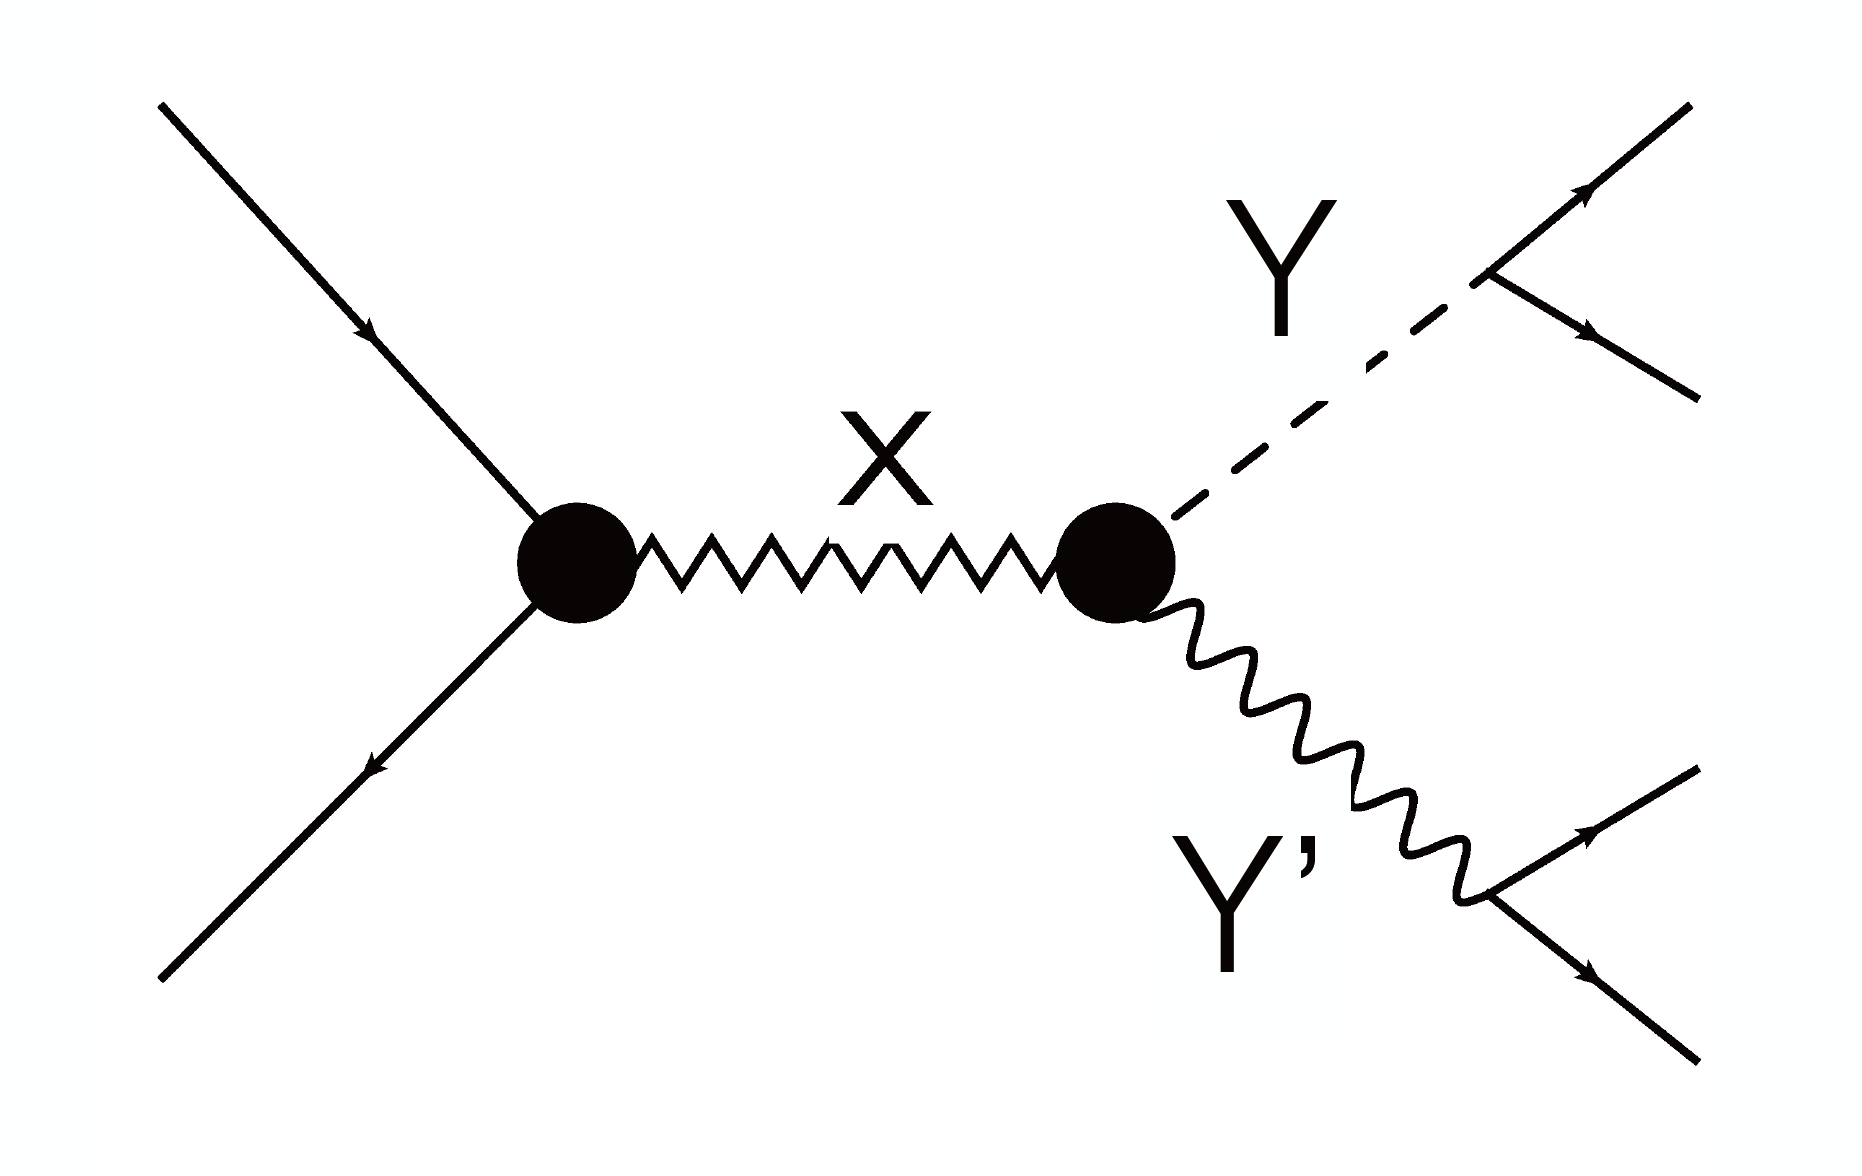
\includegraphics[height=6cm, width=10cm]{pictures/diboson_resonance_X.png}
  \caption{$X$代表TeV能量尺度的新物理粒子,$Y/Y^\prime$是$W/Z/H$玻色子。}
 \label{fig:2.9}
\end{figure}
对$X\to WW$共振态的搜寻,可以提供类似上图新物理过程的证据,发现可能的额外维度拉格朗日项、复合的希格斯粒子以及扩展的规范对称性(更多种类的$Z/W$玻色子)。
